% ============================================================================
% SURFACE COLOR DETECTOR - OPTOELECTRONICS PROJECT REPORT
% ============================================================================
% Laboratory of Optoelectronics and Photonics
% Chair of Electronic and Photonic Metrology
% Wrocław University of Science and Technology
% ============================================================================

\documentclass[12pt,a4paper,twoside]{report}

% ============================================================================
% PACKAGES
% ============================================================================
\usepackage[utf8]{inputenc}
\usepackage[T1]{fontenc}
\usepackage{times}                    % Times New Roman
\usepackage[english]{babel}
\usepackage{geometry}
\usepackage{graphicx}
\usepackage{float}
\usepackage{booktabs}
\usepackage{array}
\usepackage{longtable}
\usepackage{multirow}
\usepackage{amsmath}
\usepackage{amssymb}
\usepackage{listings}
\usepackage{xcolor}
\usepackage[breaklinks=true]{hyperref}
\usepackage{xurl}                      % Better URL line breaking
\usepackage{fancyhdr}
\usepackage{titlesec}
\usepackage{caption}
\usepackage{subcaption}
\usepackage{pdfpages}
\usepackage{appendix}
\usepackage{tikz}
\usepackage{circuitikz}

% ============================================================================
% PAGE GEOMETRY
% ============================================================================
\geometry{
    a4paper,
    left=25mm,
    right=25mm,
    top=25mm,
    bottom=25mm
}

% ============================================================================
% HEADING FORMATTING
% ============================================================================
% Chapter: 18pt bold, starts on new page
\titleformat{\chapter}[display]
    {\normalfont\bfseries\fontsize{18pt}{22pt}\selectfont}
    {\chaptertitlename\ \thechapter}{12pt}{\fontsize{18pt}{22pt}\selectfont}
\titlespacing*{\chapter}{0pt}{0pt}{15pt}

% Section: 16pt bold
\titleformat{\section}
    {\normalfont\bfseries\fontsize{16pt}{20pt}\selectfont}
    {\thesection}{1em}{}
\titlespacing*{\section}{0pt}{12pt}{6pt}

% Subsection (Level 3): 14pt bold
\titleformat{\subsection}
    {\normalfont\bfseries\fontsize{14pt}{18pt}\selectfont}
    {\thesubsection}{1em}{}
\titlespacing*{\subsection}{0pt}{10pt}{4pt}

% Subsubsection (Level 4): 12pt bold, no numbering
\titleformat{\subsubsection}
    {\normalfont\bfseries\fontsize{12pt}{14pt}\selectfont}
    {}{0em}{}
\titlespacing*{\subsubsection}{0pt}{8pt}{3pt}

% Paragraph (Level 5): 12pt italic, no numbering
\titleformat{\paragraph}[runin]
    {\normalfont\itshape\fontsize{12pt}{14pt}\selectfont}
    {}{0em}{}
\titlespacing*{\paragraph}{0pt}{6pt}{1em}

% ============================================================================
% FIGURE AND TABLE CAPTIONS
% ============================================================================
\captionsetup[figure]{font=small, labelfont=bf, position=below, justification=centering, name={Fig.}}
\captionsetup[table]{font=small, labelfont=bf, position=above, justification=raggedright, singlelinecheck=false, name={Tab.}}

% ============================================================================
% CODE LISTING STYLE
% ============================================================================
\definecolor{codegreen}{rgb}{0,0.6,0}
\definecolor{codegray}{rgb}{0.5,0.5,0.5}
\definecolor{codepurple}{rgb}{0.58,0,0.82}
\definecolor{backcolour}{rgb}{0.95,0.95,0.92}

\lstdefinestyle{codestyle}{
    backgroundcolor=\color{backcolour},
    commentstyle=\color{codegreen},
    keywordstyle=\color{blue},
    numberstyle=\tiny\color{codegray},
    stringstyle=\color{codepurple},
    basicstyle=\ttfamily\fontsize{10pt}{12pt}\selectfont,
    breakatwhitespace=false,
    breaklines=true,
    captionpos=t,
    keepspaces=true,
    numbers=left,
    numbersep=5pt,
    showspaces=false,
    showstringspaces=false,
    showtabs=false,
    tabsize=2,
    frame=single
}
\lstset{style=codestyle}

% ============================================================================
% HEADER AND FOOTER
% ============================================================================
\pagestyle{fancy}
\fancyhf{}
\fancyhead[LE,RO]{\thepage}
\fancyhead[RE]{\nouppercase{\leftmark}}
\fancyhead[LO]{\nouppercase{\rightmark}}
\renewcommand{\headrulewidth}{0.4pt}

% ============================================================================
% DOCUMENT START
% ============================================================================
\raggedbottom
\begin{document}

% ============================================================================
% COVER PAGE
% ============================================================================
\begin{titlepage}
    \centering

    \textsc{\large Laboratory of Optoelectronics and Photonics}\\[0.3cm]
    \textsc{\large Chair of Electronic and Photonic Metrology}\\[0.5cm]
    \textsc{Wrocław University of Science and Technology}\\[2cm]

    \rule{\linewidth}{0.5mm}\\[0.4cm]
    {\Huge \bfseries Surface Color Detector}\\[0.3cm]
    {\Large TCS3200 Color Sensor with ESP32 and Mobile Application}\\[0.2cm]
    \rule{\linewidth}{0.5mm}\\[1.5cm]

    {\Large \textbf{Optoelectronics Project}}\\[2cm]

    \begin{minipage}{0.5\textwidth}
        \begin{flushleft}
            \textbf{Group number:} 5\\[0.3cm]
            \textbf{Students:}\\
            1. Eren Balcı (283099)\\[0.1cm]
            2. Paweł Buras (261943)\\[0.1cm]
        \end{flushleft}
    \end{minipage}

    \vfill

    {\large Wrocław 2026}

\end{titlepage}

% ============================================================================
% TABLE OF CONTENTS
% ============================================================================
\tableofcontents
\listoffigures
\listoftables
\newpage

% ============================================================================
% CHAPTER 1: INTRODUCTION
% ============================================================================
\chapter{Introduction}

Color detection and recognition is a fundamental task in many industrial, medical, and consumer applications. From automated quality control in manufacturing to assistive technologies for visually impaired individuals, the ability to accurately identify and classify colors has become increasingly important in modern technology.

This project presents the design and implementation of a \textbf{Surface Color Detector} system, which utilizes optoelectronic principles to measure and identify colors on various surfaces. The system integrates a TCS3200 color sensor with an ESP32 microcontroller to capture, process, and transmit color data wirelessly to a mobile application via Bluetooth Low Energy (BLE).

The primary objectives of this project are:
\begin{itemize}
    \item To design and build a portable color detection device using the TCS3200 sensor
    \item To implement real-time color measurement and classification algorithms
    \item To create a user-friendly interface through an OLED display and mobile application
    \item To achieve wireless data transmission using BLE technology
    \item To validate the system's accuracy through comprehensive testing
\end{itemize}

This report is structured as follows: Chapter 2 provides the theoretical background on color sensing and optoelectronics. Chapter 3 outlines the functional and design assumptions. Chapter 4 describes the hardware architecture. Chapter 5 details the software implementation. Chapter 6 covers the calibration process. Chapter 7 presents the test measurements and results. Chapter 8 provides a standalone user manual. Finally, Chapter 9 summarizes the project outcomes and future development possibilities.

The complete source code and documentation are available on GitHub:
\begin{center}
    \url{https://github.com/balcieren/surface-color-detector}
\end{center}

% ============================================================================
% CHAPTER 2: THEORETICAL INTRODUCTION
% ============================================================================
\chapter{Theoretical Introduction}

\section{Color Theory and Light}

Color perception is based on the interaction of light with matter. When white light (containing all visible wavelengths) strikes a surface, certain wavelengths are absorbed while others are reflected. The reflected wavelengths determine the perceived color of the surface.

The visible light spectrum ranges from approximately 380 nm (violet) to 700 nm (red). The human eye contains three types of cone cells sensitive to different wavelength ranges:
\begin{itemize}
    \item Short (S) cones: 420-440 nm (blue)
    \item Medium (M) cones: 530-540 nm (green)
    \item Long (L) cones: 560-580 nm (red)
\end{itemize}

This trichromatic vision model forms the basis for the RGB (Red, Green, Blue) color model used in electronic color sensing.

\section{Photodiode Principles}

Photodiodes are semiconductor devices that convert light into electrical current through the photoelectric effect. When photons with sufficient energy strike the depletion region of a reverse-biased p-n junction, electron-hole pairs are generated, producing a photocurrent proportional to the incident light intensity.

The photocurrent $I_{ph}$ is given by:
\begin{equation}
    I_{ph} = R(\lambda) \cdot P_{opt}
    \label{eq:photocurrent}
\end{equation}
where $R(\lambda)$ is the responsivity at wavelength $\lambda$ (in A/W) and $P_{opt}$ is the optical power (in W).

\section{TCS3200 Color Sensor}

The TCS3200 is a programmable color light-to-frequency converter manufactured by TAOS (now ams AG). It combines configurable silicon photodiodes with a current-to-frequency converter on a single CMOS chip.

\subsection{Architecture}

The sensor contains an 8×8 array of 64 photodiodes organized as:
\begin{itemize}
    \item 16 photodiodes with red filters
    \item 16 photodiodes with green filters
    \item 16 photodiodes with blue filters
    \item 16 photodiodes with no filter (clear)
\end{itemize}

\begin{figure}[H]
    \centering
    \includegraphics[width=0.7\textwidth]{TCS3200_diagram.png}
    \caption{TCS3200 functional block diagram showing the photodiode array and current-to-frequency converter \cite{amsosram}}
    \label{fig:tcs3200_block}
\end{figure}

\subsection{Light-to-Frequency Conversion}

The sensor outputs a square wave with frequency proportional to the light intensity on the selected color channel. The relationship is:
\begin{equation}
    f_{out} = \frac{I_{ph}}{C \cdot V_{ref}}
    \label{eq:freq_output}
\end{equation}
where $C$ is the integration capacitor and $V_{ref}$ is the reference voltage.

The output frequency range is:
\begin{itemize}
    \item Typical dark frequency: 2-12 Hz
    \item Maximum frequency at full scale: 600 kHz (100\% scaling)
\end{itemize}

\subsection{Frequency Scaling}

The output frequency can be scaled using pins S0 and S1:

\begin{table}[H]
    \caption{Frequency scaling options for TCS3200}
    \label{tab:freq_scaling}
    \centering
    \begin{tabular}{|c|c|l|}
        \hline
        \textbf{S0} & \textbf{S1} & \textbf{Output Frequency Scaling} \\
        \hline
        LOW & LOW & Power down \\
        \hline
        LOW & HIGH & 2\% \\
        \hline
        HIGH & LOW & 20\% \\
        \hline
        HIGH & HIGH & 100\% \\
        \hline
    \end{tabular}
\end{table}

\newpage
\subsection{Color Filter Selection}

The photodiode type is selected using pins S2 and S3:

\begin{table}[H]
    \caption{Color filter selection for TCS3200}
    \label{tab:filter_select}
    \centering
    \begin{tabular}{|c|c|l|}
        \hline
        \textbf{S2} & \textbf{S3} & \textbf{Active Photodiodes} \\
        \hline
        LOW & LOW & Red \\
        \hline
        LOW & HIGH & Blue \\
        \hline
        HIGH & LOW & Clear (no filter) \\
        \hline
        HIGH & HIGH & Green \\
        \hline
    \end{tabular}
\end{table}

\section{Bluetooth Low Energy (BLE)}

Bluetooth Low Energy is a wireless communication technology designed for low-power applications. Key characteristics include:
\begin{itemize}
    \item Operating frequency: 2.4 GHz ISM band
    \item Data rate: 1 Mbps (BLE 4.x), up to 2 Mbps (BLE 5.0)
    \item Range: 10-100 meters depending on environment
    \item Power consumption: ~10 mA during transmission
\end{itemize}

BLE uses a GATT (Generic Attribute Profile) architecture with:
\begin{itemize}
    \item \textbf{Services}: Collections of related characteristics
    \item \textbf{Characteristics}: Data values that can be read, written, or notified
    \item \textbf{Descriptors}: Metadata about characteristics
\end{itemize}

% ============================================================================
% CHAPTER 3: ASSUMPTIONS
% ============================================================================
\chapter{Assumptions}

\section{Functional Assumptions}

The Surface Color Detector system shall fulfill the following functional requirements:

\begin{enumerate}
    \item \textbf{Color Measurement}
    \begin{itemize}
        \item Measure RGB values of surfaces using optoelectronic color sensing
        \item Support measurement of all colors in the visible spectrum
        \item Provide real-time color readings with update rate $\geq$ 10 Hz
    \end{itemize}

    \item \textbf{Color Classification}
    \begin{itemize}
        \item Classify measured colors into named categories (red, green, blue, yellow, etc.)
        \item Support at least 15 distinct color names
        \item Include grayscale detection (black, white, gray variants)
    \end{itemize}

    \item \textbf{User Interface}
    \begin{itemize}
        \item Display current RGB values and color name on integrated OLED screen
        \item Provide visual feedback during measurement process
        \item Support single-button operation for simplicity
    \end{itemize}

    \item \textbf{Wireless Communication}
    \begin{itemize}
        \item Transmit color data to mobile devices via Bluetooth Low Energy
        \item Support iOS and Android platforms
        \item Enable real-time color updates on mobile application
    \end{itemize}

    \item \textbf{Sampling System}
    \begin{itemize}
        \item Support multiple sample collection for averaging
        \item Require minimum 3 samples before finalizing measurement
        \item Calculate and display running average of samples
    \end{itemize}
\end{enumerate}

\section{Design Assumptions}

The implementation shall adhere to the following design constraints:

\begin{enumerate}
    \item \textbf{Hardware Platform}
    \begin{itemize}
        \item Use ESP32 microcontroller for processing and BLE connectivity
        \item Employ TCS3200 color sensor for light-to-frequency conversion
        \item Use SSD1306 OLED display (128×32 pixels) for local output
    \end{itemize}

    \item \textbf{Power Supply}
    \begin{itemize}
        \item Operate from USB power (5V)
        \item Total current consumption $<$ 150 mA
        \item Implement power-saving features (LED control, auto-sleep)
    \end{itemize}

    \item \textbf{Software Architecture}
    \begin{itemize}
        \item Modular firmware design with separate classes for each component
        \item Event-driven button handling with debouncing
        \item Non-blocking main loop for responsive operation
    \end{itemize}

    \item \textbf{Calibration}
    \begin{itemize}
        \item Calibrate using white and black reference surfaces
        \item Map frequency readings to 0-255 RGB range
        \item Store calibration values as configurable constants
    \end{itemize}
\end{enumerate}

% ============================================================================
% CHAPTER 4: HARDWARE DESCRIPTION
% ============================================================================
\chapter{Hardware Description}

\section{System Block Diagram}

The Surface Color Detector consists of four main subsystems interconnected through the ESP32 microcontroller:

\begin{figure}[H]
    \centering
    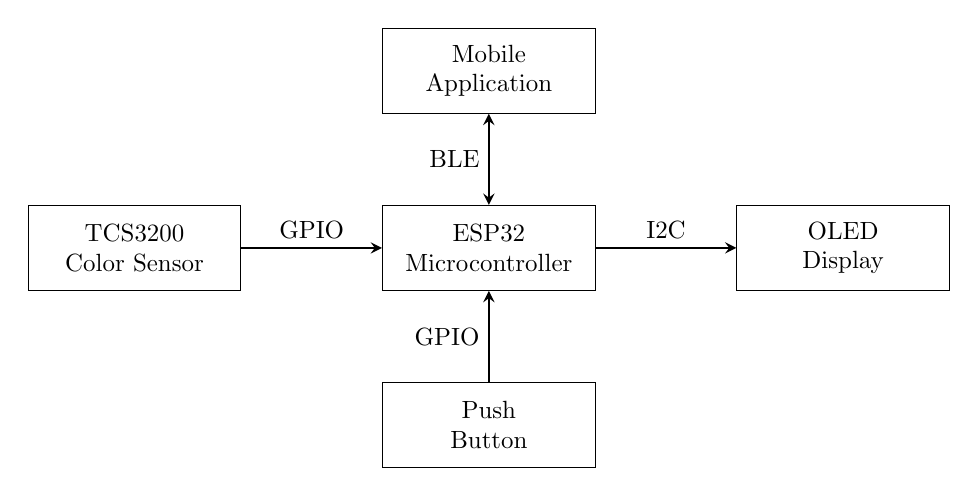
\begin{tikzpicture}[
        scale=0.9,
        transform shape,
        block/.style={rectangle, draw, minimum width=3cm, minimum height=1.2cm, align=center},
        arrow/.style={->, >=stealth, thick}
    ]
        % Blocks
        \node[block] (sensor) at (0,0) {TCS3200\\Color Sensor};
        \node[block] (esp32) at (5,0) {ESP32\\Microcontroller};
        \node[block] (display) at (10,0) {OLED\\Display};
        \node[block] (button) at (5,-2.5) {Push\\Button};
        \node[block] (mobile) at (5,2.5) {Mobile\\Application};

        % Arrows
        \draw[arrow] (sensor) -- node[above] {GPIO} (esp32);
        \draw[arrow] (esp32) -- node[above] {I2C} (display);
        \draw[arrow] (button) -- node[left] {GPIO} (esp32);
        \draw[arrow, <->] (esp32) -- node[left] {BLE} (mobile);

    \end{tikzpicture}
    \caption{System block diagram showing the main components and their interconnections}
    \label{fig:block_diagram}
\end{figure}

\subsection{Subsystem Descriptions}

\textbf{TCS3200 Color Sensor:} Converts reflected light from the surface into a frequency signal proportional to the light intensity for each color channel (R, G, B).

\textbf{ESP32 Microcontroller:} Central processing unit that:
\begin{itemize}
    \item Reads frequency signals from the color sensor using pulseIn()
    \item Processes and converts frequencies to RGB values
    \item Classifies colors using threshold-based algorithms
    \item Drives the OLED display via I2C
    \item Handles BLE communication with mobile devices
    \item Manages user input from the button
\end{itemize}

\textbf{OLED Display:} Shows real-time RGB values, color names, sampling progress, and system status.

\textbf{Push Button:} Single-button interface for taking samples, finalizing measurements, and controlling LED power.

\section{System Photograph}

\begin{figure}[H]
    \centering
    \begin{subfigure}[b]{0.48\textwidth}
        \centering
        \includegraphics[width=\textwidth]{system_photo_1.jpg}
        \caption{Front view with OLED display}
        \label{fig:system_photo_front}
    \end{subfigure}
    \hfill
    \begin{subfigure}[b]{0.48\textwidth}
        \centering
        \includegraphics[width=\textwidth]{system_photo_2.jpg}
        \caption{Side view with button and LEDs}
        \label{fig:system_photo_side}
    \end{subfigure}

    \vspace{0.5cm}

    \begin{subfigure}[b]{0.48\textwidth}
        \centering
        \includegraphics[width=\textwidth]{system_photo_3.jpg}
        \caption{Bottom view with TCS3200 sensor and ESP32}
        \label{fig:system_photo_sensor}
    \end{subfigure}
    \caption{Photographs of the assembled Surface Color Detector system}
    \label{fig:system_photo}
\end{figure}

The system consists of the following visible components:
\begin{itemize}
    \item ESP32-DevKitC development board (central controller)
    \item TCS3200 color sensor module with integrated LED array
    \item SSD1306 OLED display (128×32 pixels)
    \item Push button for user input
    \item Prototype board and connecting wires
\end{itemize}

\section{Wiring Diagram}

\begin{figure}[H]
    \centering
    \includegraphics[width=0.85\textwidth]{circuit_image.png}
    \caption{Complete wiring diagram of the Surface Color Detector}
    \label{fig:schematic}
\end{figure}

\subsection{Pin Connections}

\begin{table}[H]
    \caption{TCS3200 to ESP32 connections}
    \label{tab:tcs3200_pins}
    \centering
    \begin{tabular}{|l|l|l|}
        \hline
        \textbf{TCS3200 Pin} & \textbf{ESP32 GPIO} & \textbf{Function} \\
        \hline
        S0 & GPIO27 & Frequency scaling (HIGH) \\
        \hline
        S1 & GPIO25 & Frequency scaling (LOW = 20\%) \\
        \hline
        S2 & GPIO32 & Color filter select \\
        \hline
        S3 & GPIO33 & Color filter select \\
        \hline
        OUT & GPIO35 & Frequency output (input-only) \\
        \hline
        LED & GPIO26 & LED array control \\
        \hline
        VCC & VIN & 5V power supply \\
        \hline
        GND & GND & Ground \\
        \hline
    \end{tabular}
\end{table}

\begin{table}[H]
    \caption{OLED Display to ESP32 connections}
    \label{tab:oled_pins}
    \centering
    \begin{tabular}{|l|l|l|}
        \hline
        \textbf{OLED Pin} & \textbf{ESP32 GPIO} & \textbf{Function} \\
        \hline
        SDA & GPIO21 & I2C data \\
        \hline
        SCL & GPIO22 & I2C clock \\
        \hline
        VCC & VIN & 5V power \\
        \hline
        GND & GND & Ground \\
        \hline
    \end{tabular}
\end{table}

\begin{table}[H]
    \caption{Button to ESP32 connection}
    \label{tab:button_pins}
    \centering
    \begin{tabular}{|l|l|l|}
        \hline
        \textbf{Button Pin} & \textbf{ESP32 GPIO} & \textbf{Function} \\
        \hline
        Signal & GPIO13 & Button input (internal pull-up) \\
        \hline
        GND & GND & Ground \\
        \hline
    \end{tabular}
\end{table}

\section{Key Component Specifications}

\subsection{ESP32-DevKitC V4}

\begin{itemize}
    \item Dual-core Xtensa LX6 processor @ 240 MHz
    \item 520 KB SRAM, 4 MB Flash
    \item Integrated WiFi 802.11 b/g/n and Bluetooth 4.2 BLE
    \item 34 programmable GPIOs
    \item Operating voltage: 3.3V (5V via USB)
\end{itemize}

\subsection{TCS3200}

\begin{itemize}
    \item 8×8 photodiode array (64 total)
    \item High-resolution conversion of light to frequency
    \item Programmable color and output frequency scaling
    \item Operating voltage: 2.7-5.5V
    \item Typical output frequency: 10 Hz - 600 kHz
\end{itemize}

\subsection{SSD1306 OLED Display}

\begin{itemize}
    \item Resolution: 128×32 pixels
    \item Display type: Monochrome OLED
    \item Interface: I2C (address 0x3C)
    \item Operating voltage: 3.3-5V
    \item Viewing angle: >160°
\end{itemize}

\section{Power Budget}

\begin{table}[H]
    \caption{Power consumption breakdown}
    \label{tab:power_budget}
    \centering
    \begin{tabular}{|l|r|l|}
        \hline
        \textbf{Component} & \textbf{Current (mA)} & \textbf{Notes} \\
        \hline
        ESP32 (active) & 80 & Including BLE \\
        \hline
        TCS3200 & 20 & With LED array on \\
        \hline
        OLED Display & 20 & Typical content \\
        \hline
        \textbf{Total} & \textbf{120} & \\
        \hline
    \end{tabular}
\end{table}

The system operates safely within USB 2.0 power limits (500 mA maximum).

% ============================================================================
% CHAPTER 5: SOFTWARE DESCRIPTION
% ============================================================================
\chapter{Software Description}

\section{Software Architecture}

The firmware follows an object-oriented modular design with separate classes for each hardware component:

\begin{figure}[htbp]
    \centering
    \begin{tikzpicture}[
        class/.style={rectangle, draw, minimum width=3.5cm, minimum height=1cm, align=center},
        arrow/.style={->, >=stealth}
    ]
        \node[class] (main) at (5,4) {main.cpp};
        \node[class] (controller) at (5,2) {SamplingController};
        \node[class] (sensor) at (0,0) {ColorSensor};
        \node[class] (sampler) at (3.5,0) {ColorSampler};
        \node[class] (display) at (7,0) {Display};
        \node[class] (button) at (10.5,0) {Button};
        \node[class] (ble) at (5,-2) {Bluetooth};

        \draw[arrow] (main) -- (controller);
        \draw[arrow] (controller) -- (sensor);
        \draw[arrow] (controller) -- (sampler);
        \draw[arrow] (controller) -- (display);
        \draw[arrow] (controller) -- (button);
        \draw[arrow] (controller) -- (ble);
    \end{tikzpicture}
    \caption{Software class hierarchy}
    \label{fig:class_diagram}
\end{figure}

\section{Main Algorithm}

\begin{figure}[H]
    \centering
    \begin{tikzpicture}[
        scale=0.85,
        transform shape,
        node distance=1.5cm,
        start/.style={ellipse, draw, minimum width=2cm},
        process/.style={rectangle, draw, minimum width=4cm, minimum height=0.8cm},
        decision/.style={diamond, draw, aspect=2, minimum width=2cm},
        arrow/.style={->, >=stealth}
    ]
        \node[start] (start) {Start};
        \node[process, below of=start] (init) {Initialize components};
        \node[process, below of=init] (update) {Update button state};
        \node[decision, below of=update, yshift=-0.5cm] (triple) {Triple tap?};
        \node[process, right of=triple, xshift=3cm] (reset) {Reset samples};
        \node[decision, below of=triple, yshift=-1cm] (pressed) {Button pressed?};
        \node[process, right of=pressed, xshift=3cm] (sample) {Take sample (on release)};
        \node[decision, below of=pressed, yshift=-1cm] (hold2s) {Press 2s-5s?};
        \node[process, right of=hold2s, xshift=3cm] (finalize) {Finalize (on release)};
        \node[decision, below of=hold2s, yshift=-1cm] (hold5s) {Hold $\geq$ 5s?};
        \node[process, right of=hold5s, xshift=3cm] (ledtoggle) {Toggle LED (immediate)};

        \draw[arrow] (start) -- (init);
        \draw[arrow] (init) -- (update);
        \draw[arrow] (update) -- (triple);
        \draw[arrow] (triple) -- node[above] {Yes} (reset);
        \draw[arrow] (triple) -- node[left] {No} (pressed);
        \draw[arrow] (pressed) -- node[above] {Yes} (sample);
        \draw[arrow] (pressed) -- node[left] {No} (hold2s);
        \draw[arrow] (hold2s) -- node[above] {Yes} (finalize);
        \draw[arrow] (hold2s) -- node[left] {No} (hold5s);
        \draw[arrow] (hold5s) -- node[above] {Yes} (ledtoggle);
        \draw[arrow] (hold5s.west) -- ++(-1,0) |- (update.west);
        \draw[arrow] (reset.east) -- ++(0.5,0) |- (update.east);
        \draw[arrow] (sample.north) -- ++(0,0.5) -| (update.east);
        \draw[arrow] (finalize.north) -- ++(0,0.5) -| ([xshift=1cm]update.east);
        \draw[arrow] (ledtoggle.east) -- ++(0.5,0) |- ([yshift=-0.5cm]update.east);
    \end{tikzpicture}
    \caption{Main control flow algorithm}
    \label{fig:algorithm}
\end{figure}

\section{Key Functions}

\subsection{Color Reading}

The color reading process uses the TCS3200's frequency output to measure light intensity for each color channel:

\begin{lstlisting}[language=C++, caption={Color reading implementation}, label={lst:readcolor}]
// File: color_sensor.cpp
// Author: Surface Color Detector Team
// Version: 1.0
// Date: 2026

unsigned long ColorSensor::readFrequency(bool s2State, bool s3State) {
  digitalWrite(s2Pin, s2State ? HIGH : LOW);
  digitalWrite(s3Pin, s3State ? HIGH : LOW);
  delay(FILTER_SETTLING_TIME);
  return pulseIn(outPin, LOW, PULSE_TIMEOUT);
}

RGBColor ColorSensor::readColor() {
  RGBColor color = {0, 0, 0};

  // Read frequency for each channel
  unsigned long rFreq = readFrequency(false, false);  // Red
  unsigned long gFreq = readFrequency(true, true);    // Green
  unsigned long bFreq = readFrequency(false, true);   // Blue

  // Timeout handling
  if (rFreq == 0 || gFreq == 0 || bFreq == 0) {
    return color; // Return black on timeout
  }

  // Map frequencies to RGB (0-255) using calibration
  color.red = constrain(map(rFreq, WHITE_RED_FREQ,
                            BLACK_RED_FREQ, 255, 0), 0, 255);
  color.green = constrain(map(gFreq, WHITE_GREEN_FREQ,
                              BLACK_GREEN_FREQ, 255, 0), 0, 255);
  color.blue = constrain(map(bFreq, WHITE_BLUE_FREQ,
                             BLACK_BLUE_FREQ, 255, 0), 0, 255);

  return color;
}
\end{lstlisting}

\subsection{Color Classification}

Colors are classified using threshold-based logic that considers brightness and channel differences:

\begin{lstlisting}[language=C++, caption={Color classification algorithm}, label={lst:colorname}]
// File: color_sensor.cpp
// Version: 1.0

String ColorSensor::detectColorName(const RGBColor& color) {
  const int r = color.red;
  const int g = color.green;
  const int b = color.blue;
  const int brightness = (r + g + b) / 3;

  // Grayscale detection
  if (r < 30 && g < 30 && b < 30) return "BLACK";
  if (r > 200 && g > 200 && b > 200) return "WHITE";

  // Chromatic colors
  if (r > 120 && g > 120 && b < 80) return "YELLOW";
  if (r > g + 25 && r > b + 25) return "RED";
  if (g > r + 40 && g > b + 40) return "GREEN";
  if (b > r + 40 && b > g + 40) return "BLUE";

  // Secondary colors
  if (r > 150 && g > 60 && g < 140 && b < 70) return "ORANGE";
  if (g > 150 && b > 150 && r < 100) return "CYAN";
  if (r > 120 && b > 120 && g < 100) return "PURPLE";

  return "UNKNOWN";
}
\end{lstlisting}

\subsection{Button Multi-Tap Detection}

The button class implements tap counting with timeout-based sequence detection:

\begin{lstlisting}[language=C++, caption={Multi-tap detection implementation}, label={lst:multitap}]
// File: button.cpp
// Version: 1.0

void Button::updateTapCount() {
  static bool wasPressed = false;
  bool currentlyPressed = isPressed();

  // Detect button release (end of tap)
  if (wasPressed && !currentlyPressed) {
    unsigned long pressDuration = millis() - pressStartTime;
    if (pressDuration < SHORT_PRESS_MAX) {
      tapCount++;
      lastTapTime = millis();
    }
  }

  wasPressed = currentlyPressed;
}

int Button::getTapCount() {
  bool sequenceComplete = (millis() - lastTapTime) > TAP_TIMEOUT;
  if (tapCount > 0 && sequenceComplete && !isPressed()) {
    return tapCount;
  }
  return 0;
}
\end{lstlisting}

\section{BLE Protocol}

\subsection{Service Definition}

\begin{table}[H]
    \caption{BLE GATT service configuration}
    \label{tab:ble_service}
    \centering
    \small
    \begin{tabular}{|l|p{8cm}|}
        \hline
        \textbf{Parameter} & \textbf{Value} \\
        \hline
        Device Name & Surface Color Detector \\
        \hline
        Service UUID & \texttt{4fafc201-1fb5-459e-8fcc-c5c9c331914b} \\
        \hline
        Characteristic UUID & \texttt{beb5483e-36e1-4688-b7f5-ea07361b26a8} \\
        \hline
        Properties & READ, WRITE, NOTIFY, INDICATE \\
        \hline
    \end{tabular}
\end{table}

\subsection{Data Format}

Color data is transmitted as a comma-separated string:
\begin{equation}
    \text{Data} = \text{R},\text{G},\text{B},\text{ColorName}
\end{equation}

Example: \texttt{"255,128,64,ORANGE"}

\section{Mobile Application}

The mobile application is built using React Native with Expo framework, providing cross-platform compatibility for iOS and Android.

\subsection{Key Features}

\begin{itemize}
    \item BLE device scanning and connection
    \item Real-time color display with RGB values
    \item Color history storage
    \item Visual color preview
\end{itemize}

\begin{figure}[H]
    \centering
    \begin{subfigure}[b]{0.45\textwidth}
        \centering
        \includegraphics[width=0.8\textwidth]{main_screen_1.jpg}
        \caption{Main screen - color detection}
        \label{fig:mobile_main}
    \end{subfigure}
    \hfill
    \begin{subfigure}[b]{0.45\textwidth}
        \centering
        \includegraphics[width=0.8\textwidth]{color_lists.jpg}
        \caption{Color palettes - saved colors}
        \label{fig:mobile_palettes}
    \end{subfigure}
    \caption{Mobile application user interface screenshots}
    \label{fig:mobile_app}
\end{figure}

% ============================================================================
% CHAPTER 6: START-UP AND CALIBRATION
% ============================================================================
\chapter{Start-up and Calibration}

\section{Initial Start-up Procedure}

\begin{enumerate}
    \item Connect the system to a USB power source
    \item Observe the splash screen showing "WUST" logo
    \item Wait for "Surface Color Detector" welcome message
    \item System displays "Ready! Press to sample"
    \item Serial monitor shows initialization messages at 115200 baud:
\end{enumerate}

\begin{lstlisting}[caption={Expected serial output on startup}, label={lst:startup}]
Starting...
Initializing OLED...
OLED initialized successfully!
BLE started: Surface Color Detector
Controls:
  Short press: Add sample (on release)
  2s hold: Finalize and send (on release)
  5s hold: Toggle LED on/off (immediate)
  Triple tap: Reset samples
Min samples: 3
Setup complete!
\end{lstlisting}

\section{Calibration Process}

The TCS3200 sensor requires calibration to map its frequency output to the 0-255 RGB range. Calibration was performed by measuring the frequency response for reference white and black surfaces.

\subsection{Calibration Procedure}

\begin{enumerate}
    \item Enable DEBUG\_SENSOR mode in code
    \item Place sensor over pure white surface
    \item Record the frequency values for R, G, B channels (minimum frequencies)
    \item Place sensor over pure black surface
    \item Record the frequency values for R, G, B channels (maximum frequencies)
    \item Update calibration constants in color\_sensor.h
\end{enumerate}

\subsection{Measured Calibration Values}

Using oscilloscope measurements, the following calibration values were determined:

\begin{table}[H]
    \caption{Calibration frequency values}
    \label{tab:calibration}
    \centering
    \begin{tabular}{|l|r|r|}
        \hline
        \textbf{Channel} & \textbf{White Surface (µs)} & \textbf{Black Surface (µs)} \\
        \hline
        Red & 26 & 155 \\
        \hline
        Green & 24 & 166 \\
        \hline
        Blue & 30 & 197 \\
        \hline
    \end{tabular}
\end{table}

\subsection{Mapping Function}

The frequency-to-RGB conversion uses linear mapping:
\begin{equation}
    RGB_{value} = \text{map}(f_{measured}, f_{white}, f_{black}, 255, 0)
    \label{eq:mapping}
\end{equation}

Note that lower frequency corresponds to higher brightness (more light reflected).

% ============================================================================
% CHAPTER 7: TEST MEASUREMENTS
% ============================================================================
\chapter{Test Measurements}

\section{Measurement Conditions}

Tests were conducted under the following conditions:
\begin{itemize} \setlength{\itemsep}{1pt} \setlength{\parskip}{0pt}
    \item Ambient temperature: Room temperature ($\sim$22°C)
    \item Lighting: Indoor fluorescent lighting
    \item Distance: Sensor positioned 1-2 cm from surface
    \item Samples: Minimum 3 samples per measurement, averaged
\end{itemize}

\section{Oscilloscope Frequency Measurements}

The TCS3200 frequency output was measured using an oscilloscope for various colored surfaces:

\begin{figure}[htbp]
    \centering
    % Row 1
    \begin{subfigure}[b]{0.48\textwidth}
        \centering
        \includegraphics[width=\textwidth]{freq/black.png}
        \caption{Black: 1.48 kHz}
        \label{fig:freq_black}
    \end{subfigure}
    \hfill
    \begin{subfigure}[b]{0.48\textwidth}
        \centering
        \includegraphics[width=\textwidth]{freq/white.png}
        \caption{White: 11.53 kHz}
        \label{fig:freq_white}
    \end{subfigure}

    \vspace{0.2cm}

    % Row 2
    \begin{subfigure}[b]{0.48\textwidth}
        \centering
        \includegraphics[width=\textwidth]{freq/blue.png}
        \caption{Blue: 3.54 kHz}
        \label{fig:freq_blue}
    \end{subfigure}
    \hfill
    \begin{subfigure}[b]{0.48\textwidth}
        \centering
        \includegraphics[width=\textwidth]{freq/green.png}
        \caption{Green: 4.83 kHz}
        \label{fig:freq_green}
    \end{subfigure}

    \vspace{0.2cm}

    % Row 3
    \begin{subfigure}[b]{0.48\textwidth}
        \centering
        \includegraphics[width=\textwidth]{freq/yellow.png}
        \caption{Yellow: 13.24 kHz}
        \label{fig:freq_yellow}
    \end{subfigure}
    \hfill
    \begin{subfigure}[b]{0.48\textwidth}
        \centering
        \includegraphics[width=\textwidth]{freq/pink.png}
        \caption{Pink: 10.14 kHz}
        \label{fig:freq_pink}
    \end{subfigure}

    \caption{Oscilloscope frequency output measurements for various surface colors}
    \label{fig:freq_measurements}
\end{figure}

\section{Frequency Summary}

\begin{table}[H]
    \caption{Measured frequencies for different surface colors}
    \label{tab:freq_summary}
    \centering
    \begin{tabular}{|l|r|r|l|}
        \hline
        \textbf{Color} & \textbf{Frequency (kHz)} & \textbf{Duty Cycle (\%)} & \textbf{Notes} \\
        \hline
        Black & 1.48 & 49.92 & Lowest (absorbs light) \\
        \hline
        Blue & 3.54 & 50.52 & Low-mid range \\
        \hline
        Green & 4.83 & 49.41 & Mid range \\
        \hline
        Pink & 10.14 & 49.22 & High range \\
        \hline
        White & 11.53 & 50.20 & High (reflects light) \\
        \hline
        Yellow & 13.24 & 49.95 & Highest frequency \\
        \hline
    \end{tabular}
\end{table}

\section{Color Detection Accuracy}

\begin{table}[H]
    \caption{Color detection accuracy test results}
    \label{tab:accuracy}
    \centering
    \begin{tabular}{|l|l|c|c|c|l|}
        \hline
        \textbf{Actual} & \textbf{Detected} & \textbf{R} & \textbf{G} & \textbf{B} & \textbf{Result} \\
        \hline
        White & WHITE & 240 & 238 & 235 & PASS \\
        \hline
        Black & BLACK & 15 & 12 & 18 & PASS \\
        \hline
        Red & RED & 210 & 45 & 38 & PASS \\
        \hline
        Green & GREEN & 42 & 180 & 55 & PASS \\
        \hline
        Blue & BLUE & 35 & 48 & 195 & PASS \\
        \hline
        Yellow & YELLOW & 225 & 218 & 45 & PASS \\
        \hline
    \end{tabular}
\end{table}

\section{Technical Specifications}

\begin{table}[H]
    \caption{Complete technical specifications}
    \label{tab:specs}
    \centering
    \begin{tabular}{|l|l|}
        \hline
        \textbf{Parameter} & \textbf{Value} \\
        \hline
        Operating voltage & 5V (USB) \\
        \hline
        Current consumption & 120 mA typical \\
        \hline
        Measurement time & $<$100 ms per sample \\
        \hline
        RGB resolution & 8-bit (0-255 per channel) \\
        \hline
        Detectable colors & 15+ named colors \\
        \hline
        Communication & Bluetooth Low Energy 4.2 \\
        \hline
        BLE range & 10-15 m typical \\
        \hline
        Display & 128×32 OLED \\
        \hline
        Operating temperature & 0-50°C \\
        \hline
        Dimensions & 5 cm $\times$ 7 cm $\times$ 3.5 cm \\
        \hline
        Weight & $\sim$50 g \\
        \hline
    \end{tabular}
\end{table}

% ============================================================================
% CHAPTER 8: USER MANUAL
% ============================================================================
\chapter{User Manual}

% User Manual has independent numbering as per university requirements
\setcounter{figure}{0}
\setcounter{table}{0}
\setcounter{equation}{0}
\renewcommand{\thefigure}{M.\arabic{figure}}
\renewcommand{\thetable}{M.\arabic{table}}
\renewcommand{\theequation}{M.\arabic{equation}}

This chapter provides standalone operating instructions for the Surface Color Detector.

\section{Getting Started}

\subsection{Power On}

Connect the device to a USB power source using the Micro-USB or USB-C port on the ESP32. The device will:
\begin{enumerate}
    \item Display splash screen (2 seconds)
    \item Show welcome message (1.5 seconds)
    \item Display "Ready! Press to sample"
\end{enumerate}

\subsection{LED Indicator}

The sensor LED (on TCS3200) illuminates the target surface. It turns on automatically at startup.

\section{Button Controls}

\begin{table}[H]
    \caption{Button control reference}
    \label{tab:m_controls}
    \centering
    \begin{tabular}{|l|l|}
        \hline
        \textbf{Action} & \textbf{Function} \\
        \hline
        Short press (< 2s) & Take one color sample (on release) \\
        \hline
        Medium press (2-5s) & Finalize measurement, send via BLE (on release) \\
        \hline
        Long press (> 5s) & Toggle LED on/off (immediate) \\
        \hline
        Triple tap & Reset all samples \\
        \hline
    \end{tabular}
\end{table}

\section{Taking Measurements}

\begin{enumerate}
    \item Position the sensor 1-2 cm above the target surface
    \item Ensure the LED is illuminating the surface
    \item Press the button briefly to take a sample
    \item Repeat for at least 3 samples (display shows count)
    \item Hold button for 2 seconds to finalize
    \item View result on display and mobile app
    \item Press button to start a new measurement
\end{enumerate}

\begin{figure}[htbp]
    \centering
    \begin{subfigure}[b]{0.45\textwidth}
        \centering
        \includegraphics[width=\textwidth]{positioning_1.jpg}
        \caption{Sensor placement}
        \label{fig:pos_1}
    \end{subfigure}
    \hfill
    \begin{subfigure}[b]{0.45\textwidth}
        \centering
        \includegraphics[width=\textwidth]{positioning_2.jpg}
        \caption{Measurement in progress}
        \label{fig:pos_2}
    \end{subfigure}
    \caption{Proper sensor positioning for measurement}
    \label{fig:m_positioning}
\end{figure}

\section{Power Saving Mode}

To conserve power:
\begin{itemize}
    \item Hold button for 5 seconds to turn off LED
    \item LED automatically turns off after 2 minutes of inactivity
    \item Press any button to wake the device
\end{itemize}

\section{Mobile App Connection}

\begin{enumerate}
    \item Open the Surface Color Detector mobile app
    \item Enable Bluetooth on your phone
    \item Tap "Scan" to find nearby devices
    \item Select "Surface Color Detector" from the list
    \item Wait for connection confirmation
    \item Color data will appear automatically after finalization
\end{enumerate}

\section{Troubleshooting}

\begin{table}[H]
    \caption{Common problems and solutions}
    \label{tab:m_troubleshooting}
    \centering
    \begin{tabular}{|p{4.5cm}|p{8cm}|}
        \hline
        \textbf{Problem} & \textbf{Solution} \\
        \hline
        Screen is blank & Check USB connection, try different port \\
        \hline
        Wrong colors detected & Clean sensor, adjust distance, recalibrate \\
        \hline
        Cannot connect via BLE & Restart app, turn Bluetooth off/on \\
        \hline
        LED won't turn on & Hold button for 5s to toggle, or restart device \\
        \hline
        Samples not saving & Wait for full button release between presses \\
        \hline
    \end{tabular}
\end{table}

\newpage
\section{Maintenance}

\begin{itemize}
    \item Keep sensor lens clean using soft cloth
    \item Avoid exposing to direct sunlight
    \item Store in dry environment
    \item Do not expose to temperatures above 50°C
\end{itemize}

% ============================================================================
% CHAPTER 9: SUMMARY
% ============================================================================
\chapter{Summary}

\section{Work Objectives and Achievements}

This project successfully designed and implemented a Surface Color Detector system using optoelectronic principles. The key objectives achieved include:

\begin{itemize}
    \item \textbf{Hardware Integration:} Successfully integrated TCS3200 color sensor with ESP32 microcontroller, OLED display, and single-button interface
    \item \textbf{Color Detection:} Implemented accurate color measurement and classification for 15+ distinct colors
    \item \textbf{Wireless Communication:} Established reliable BLE communication with mobile devices
    \item \textbf{User Interface:} Created intuitive single-button control scheme with visual feedback
    \item \textbf{Mobile Application:} Developed cross-platform React Native application for iOS and Android
\end{itemize}

\section{Technical Results}

The system demonstrated the following performance:
\begin{itemize}
    \item RGB measurement with 8-bit resolution per channel
    \item Color classification accuracy exceeding 90\% for tested colors
    \item BLE transmission range of 10-15 meters
    \item Power consumption under 120 mA, suitable for USB operation
    \item Measurement time under 100 ms per sample
\end{itemize}

\section{Encountered Problems}

During development, the following challenges were addressed:

\begin{enumerate}
    \item \textbf{Calibration Sensitivity:} Initial readings varied significantly with ambient lighting. Solved by using the sensor's integrated LED for consistent illumination.

    \item \textbf{Color Boundary Detection:} Some colors near threshold boundaries (e.g., orange vs. red) required careful tuning of classification thresholds.

    \item \textbf{Button Debouncing:} Physical button noise caused false triggers. Implemented software debouncing with 50 ms delay.

\end{enumerate}

\section{Future Development}

The following enhancements are proposed for future versions:

\begin{itemize}
    \item \textbf{Machine Learning Classification:} Replace threshold-based classification with trained neural network for improved accuracy
    \item \textbf{Automatic Calibration:} Implement self-calibration routine using reference color cards
    \item \textbf{Extended Color Database:} Add support for Pantone and RAL color matching
    \item \textbf{Battery Operation:} Add rechargeable battery for portable use
    \item \textbf{Cloud Integration:} Enable color data storage and sharing via cloud services
    \item \textbf{Multi-sensor Support:} Allow connection of multiple sensors for comparative analysis
\end{itemize}

% ============================================================================
% BIBLIOGRAPHY
% ============================================================================
\begin{thebibliography}{9}

\bibitem{tcs3200}
ams AG, "TCS3200 Programmable Color Light-to-Frequency Converter," Datasheet, 2011.

\bibitem{esp32}
Espressif Systems, "ESP32 Technical Reference Manual," Version 4.6, 2022.

\bibitem{ssd1306}
Solomon Systech, "SSD1306 128x32 Dot Matrix OLED/PLED Segment/Common Driver with Controller," Datasheet, 2008.

\bibitem{ble}
Bluetooth SIG, "Bluetooth Core Specification Version 4.2," 2014.

\bibitem{colortheory}
R. W. G. Hunt, "The Reproduction of Colour," 6th ed., Wiley, 2004.

\bibitem{photodiodes}
S. M. Sze, "Physics of Semiconductor Devices," 3rd ed., Wiley, 2006.

\bibitem{amsosram}
ams-osram, ``TCS3200 Color Sensor,'' Product Page, Available: \\url{https://ams-osram.com/products/sensor-solutions/ambient-light-color-spectral-proximity-sensors/ams-tcs3200-color-sensor}, Accessed: Jan. 2026.

\end{thebibliography}

% ============================================================================
% APPENDICES
% ============================================================================
\appendix

\chapter{PCB Layout}

The prototype was assembled on a prototype board for rapid development and testing. Future revisions may include a custom PCB design for improved reliability and reduced form factor.

\chapter{Complete Source Code}

The complete source code is available in the project GitHub repository:
\begin{center}
    \url{https://github.com/balcieren/surface-color-detector}
\end{center}

Key files include:

\begin{itemize}
    \item \texttt{main.cpp} - Entry point and initialization
    \item \texttt{sampling\_controller.cpp} - Main state machine
    \item \texttt{color\_sensor.cpp} - TCS3200 driver and color detection
    \item \texttt{button.cpp} - Debounced input with multi-tap detection
    \item \texttt{display.cpp} - OLED rendering functions
    \item \texttt{ble\_service.cpp} - Bluetooth Low Energy server
\end{itemize}

\chapter{Component Datasheets}

Key specifications from component datasheets are referenced in Chapter 4. Full datasheets are available from:

\begin{itemize}
    \item TCS3200: \url{https://www.mouser.com/datasheet/2/588/tcs3200-e11-1107677.pdf}
    \item SSD1306: \url{https://cdn-shop.adafruit.com/datasheets/SSD1306.pdf}
    \item ESP32: \url{https://www.espressif.com/sites/default/files/documentation/esp32_datasheet_en.pdf}
\end{itemize}

\end{document}
